\documentclass[12pt]{article}
\usepackage[utf8]{inputenc}

\usepackage[symbol]{footmisc} % footnote symbols

\usepackage{graphicx}
\graphicspath{ {output/} } % compile mode must be normal for images to display

\usepackage[
    letterpaper, 
    portrait, 
    margin=1in]{geometry} % set paper size, orientation, and margins
    
\usepackage[
    backend=biber,
    style=apa]{biblatex} % Imports biblatex package
    
\addbibresource{ref.bib} % Import the bibliography file

% set line spacing
\setlength{\parindent}{3em}
\setlength{\parskip}{0em}
\renewcommand{\baselinestretch}{1.5}

\renewcommand{\thefootnote}{\fnsymbol{footnote}}




\begin{document}

\hspace{5pt}

\Large
 \begin{center}
High-Resolution Estimates of Agricultural Land Value for Conservation\footnote[2]{Gold and Binder acknowledge financial support from the David \& Lissa Leege Endowment and professional development grant funds from the Faculty Life Committee of St Olaf College. They would also like to thank Rushikesh Jadhav for research assistance and Sara Dale and Craig Rice for their indispensable technical assistance.}\\ 
% I need to verify that I'm acknowledging the funding sources properly.

\vspace{10pt}

% Authors
\large
Asa Gold$^1$, Seth Binder$^1$, Christoph Nolte$^2$ \\

\vspace{10pt}

\footnotesize  
$^{1}$St. Olaf College\\
$^2$Boston University

\vspace{40pt} 

    \normalsize
    \textbf{Abstract}
\end{center}

\small
Planning for cost-effective conservation requires reliable estimates of land costs, spatially-differentiated at high resolution. Nolte (2020) provides an estimation approach that dramatically improves estimates for undeveloped land. Much undeveloped land of conservation interest is under threat of conversion to agricultural use or is already agricultural. Here we improve on the accuracy and coverage of estimation models for such land by incorporating additional variables known to affect agricultural land value and by modeling at scales corresponding to regional agricultural markets. Our estimates improve accuracy by X percent on average and extend coverage by Y percent. 

\newpage

Agencies and private organizations designing conservation efforts must contend with the fundamental scarcity of available resources, while simultaneously confronting a vast array of potential conservation strategies. Accurately predicting costs of competing strategies, then, is crucial to achieving the cost-effective use of scarce conservation dollars. The value of land is the primary determinant of such costs. Yet, academics and planners have not often had access to reliable estimates of fair market land value. Some studies have relied on state or county-wide average land value estimates [e.g., Withey 2012, Lawler 2020], which obscure important heterogeneity of land values across those geographically large political units. Recent work suggests that conservation strategies based on such low-resolution cost estimates can substantially underestimate the cost of selected plans (\cite{Nolte2020High-resolutionStates}). 

Several studies aim at providing more accurate, higher-resolution land value estimates with national coverage. Larson (2015) uses a patchwork of USDA county-level agricultural land value estimates and existing hedonic estimates of urban land value (Kuminoff and Pope 2013) to interpolate values to a mix of parcels, census tracts, and counties across the contiguous U.S. Albouy et al (2017) estimate urban land values for every Metropolitan Statistical Area (MSA) in the U.S. For each MSA, they leverage sales data from the CoStar COMPS database to estimate land value per acre as a continuous function of distance from the city center. The majority of conservation interest, of course, lies outside of urban areas. With a primary focus on undeveloped land, Nolte (2020) integrates a nationwide database of parcel-specific information, including location, built environment, local demographics, and physical landscape features, with Zillow’s ZTRAX database of millions of sales records for use in a machine-learning algorithm to estimate land values at much higher spatial resolution. These estimates explain a much greater portion of observed variation in sales value than county-wide averages. The Nolte approach constitutes a leap forward for estimating the value of undeveloped land value for conservation planning. As we show here, it can be further improved.

Accurately predicting the value of agricultural (or potentially agricultural) land is particularly important. Such land is a primary target for conservation advocates, either as a bulwark against further development or to recover natural ecosystems from degrading agricultural practices, such as monocropping [need citation here]. But because farmland value does not exhibit dynamics identical to those of other land types, appraisals that do not address agricultural property as a unique category might fail to accurately portray the costs of bringing farmland (or other arable land) under the aegis of regulatory agencies or non-profits like The Nature Conservancy. In Nolte's (2020) analysis, the massive scope does not treat the drivers of agricultural land value as distant from other land types.

There is reason to believe that expanding the set of agriculturally and economically relevant predictors as well as the geographic scale of analysis could improve the coverage and quality of land value estimates. The market value of undeveloped land is in many cases driven by the value of its actual or potential use in agriculture. It can also be driven by demand in related, residential land markets. Climate and soil variables, heretofore absent from the list of Nolte predictors, are well known to be important determinants of agricultural productivity and land value [citations]. Irrigation can also be an important determinant of productivity for particular crops and geographies, though it requires costly investment. The irrigation status of land can indicate unobserved investments in machinery, infrastructure or physical changes to land that enhance its market value. 

While many of the land quality attributes that determine economic value are fixed, or change only very slowly over time, many drivers of supply and demand—income, preferences, technology, and the availability of substitutes---vary over time. Home price indices capture changing dynamics in residential land markets that can exert pressure on (or otherwise correlate with) the price of undeveloped land. Accounting for variation in local home prices might thus improve the predictive power of models aimed at estimating the value of agricultural or other undeveloped land. 

In addition to incorporating additional predictors, we consider the possibility that modeling at scales larger than the county can ease local observation constraints, improving both the coverage and accuracy of resulting estimates. Many counties have few sales records in the ZTRAX database. Nolte (2020) implements a 1000-observation minimum for modeling county land values, supplementing a focal county’s observations with observations drawn from neighboring counties where possible. Even with this supplementation procedure, x percent of counties fail to meet the threshold, and prediction accuracies for counties with sufficient-but-low observation densities are notably poorer than those for other counties. We propose modeling at the larger scale of USDA farm resource regions, which are delineated in consideration of similarities in geography and agricultural production \textbf{Add citation for (USDA 2000)}.

BRIEF OVERVIEW OF RESULTS W/ REFERENCE TO SECTIONS? 


\section{Data and Methods}
We base our analysis on data first published by Nolte (2020), a comprehensive high-resolution dataset of parcel characteristics and sales across the contiguous United States (140.9 million properties across 3,055 counties), including variables on building presence, development, accessibility, local demographics, local nature preservation, terrain, water, flood risk, land cover type, location, and date of sale. To these base data, we add variables for soil quality, climate, irrigation status, and local real estate prices.

Soil classifications, indicating a map unit's suitability for agricultural use, were compiled from the Natural Resources Conservation Service (NRCS)’s high-resolution SSURGO soil survey database (\cite{SoilSurveyStaffSoilStates}). The NRCS soil survey provides map unit polygons that describe soil components (e.g., ``loamy fine sand, 0 to 2 percent slopes") and characteristics, including water capacity, flooding frequency, farmland classification, and features limiting development, among others. Soil farmland classifications indicate a map unit's suitability for agriculture fall under five general classes, defined by the USDA:
\begin{enumerate}
    \item Prime, optimal site composition and availability for producing agricultural product;  
    \item Unique, soil producing high-value crops (e.g., vineyards in California); 
    \item Statewide Importance, state-defined agricultural land that fails to meet prime criteria;
    \item Local importance, locally defined agricultural land that fails to meet prime or statewide criteria
    \item Conditional classes, land that would be considered prime, statewide importance, or local importance conditional on a specified improvement (e.g., ``Prime if drained and protected from flooding")
\end{enumerate}

Farmland classifications are operationalized as the percent of each parcel containing a given classification (e.g., ``Prime Farmland” or ``Farmland of Statewide Importance”). Aggregation is applied to overlapping classifications containing multiple conditions. For instance, ``Prime if drained or protected from flooding" gets assigned to ``Prime if drained" and ``Prime if protected from flooding." 

30-year, monthly climate normals of minimum, mean, and maximum temperature, as well as dew temperature and precipitation come from the PRISM Climate Group (\cite{PRISMClimate2021}). We aggregate these to the meteorological season. Parcel irrigation status is based on annual 1997-2017 estimates at a resolution of 30 sq. meters, produced by the Landsat-based Irrigation Dataset, or LANID-US (\cite{Xie2021MappingStates}). We create two binary irrigation variables to record 1) whether the parcel had ever been irrigated prior to sale, and 2) whether it was irrigated at any point in the 3 years immediately preceding the sale. 

To incorporate information on local real estate markets, we add yearly all-transaction house price index values at the county level (\cite{FederalHousing2022}).

To focus our analysis on agricultural land value, we filter the ZTRAX data to only include parcels that are undeveloped, agricultural, or potentially agricultural (see Appendix for complete filtering criteria).
Our filter results in 5.26 million unique sales observations nationwide, split into testing (\textit{n = 1.47 million}) and training (\textit{n = 3.78 million}) sets stratified along the outcome variable (Fig. \ref{fig:train_test}).

\begin{figure}
    \centering
    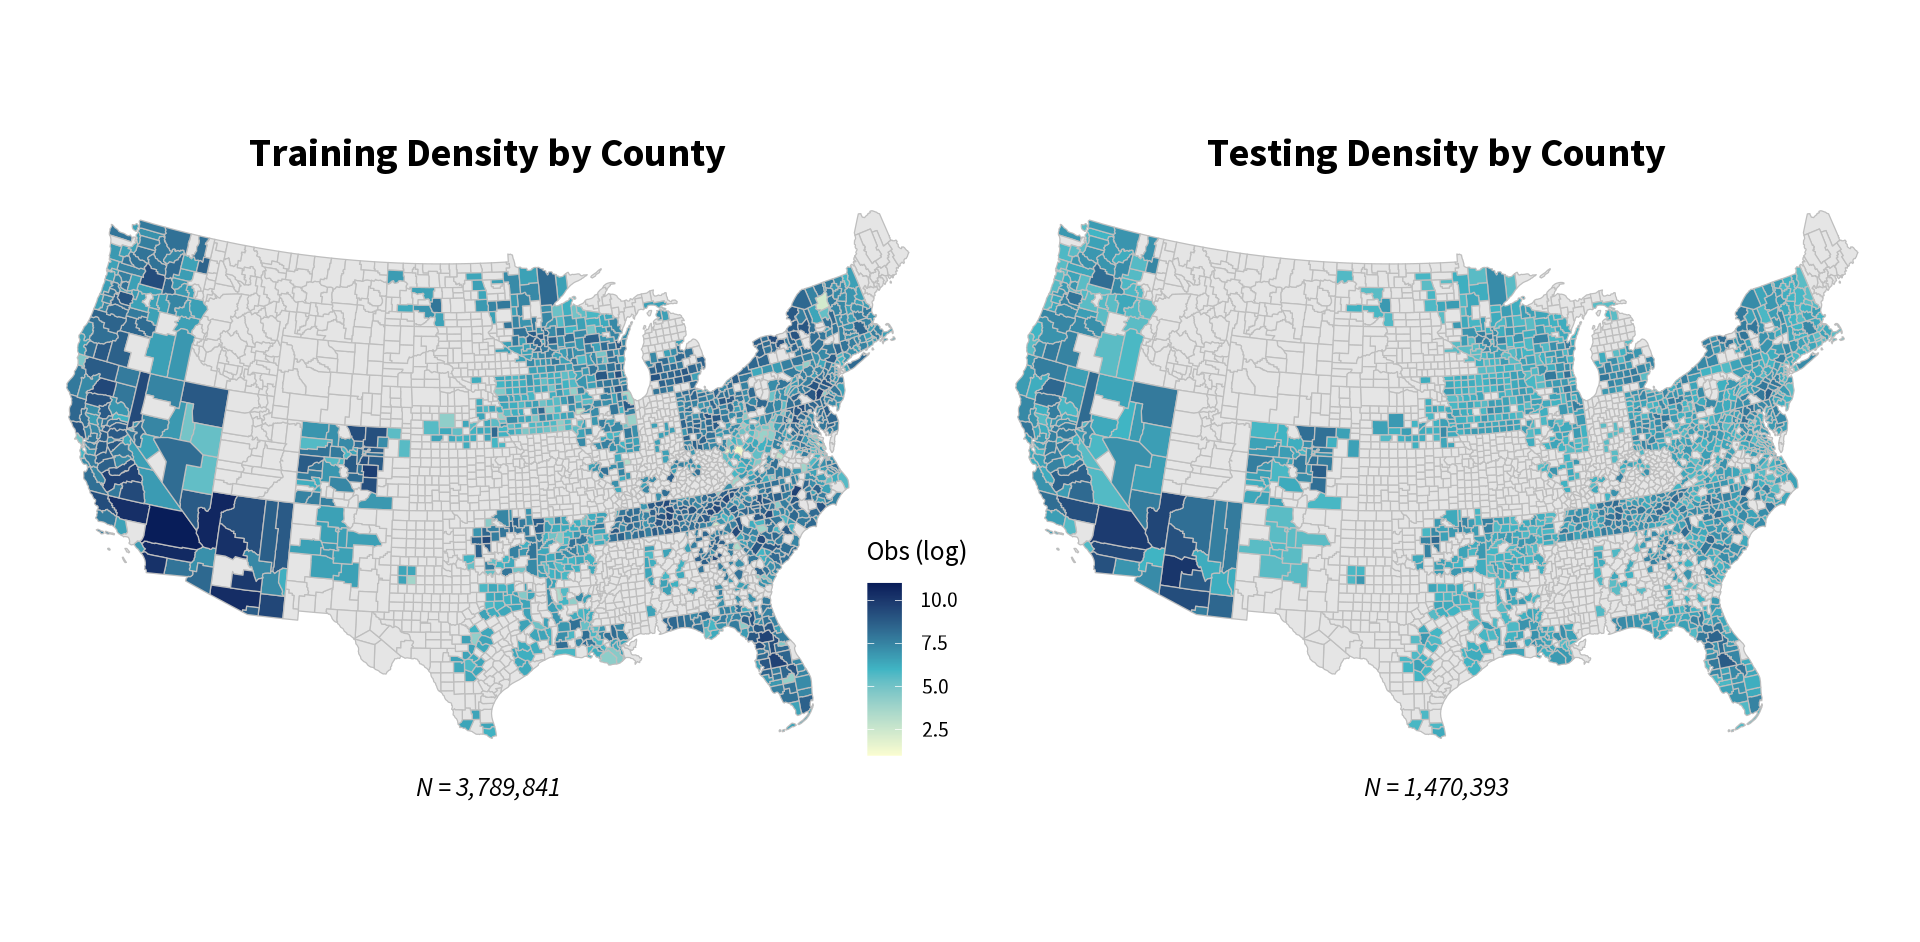
\includegraphics[width=6in]{figures/test_train_density.png}
    \caption{Observation density by training and testing sets}
    \label{fig:train_test}
\end{figure}

With this expanded dataset, we model the fair market value of parcels--measured as logged per-hectare price, adjusted for inflation using monthly consumer price index (CPI) values (\cite{blsConsumerPrice})--in two ways: linear regression and extremely randomized trees, a decision tree-based bagging algorithm. We compare these statistical approaches based on predictive accuracy, explanatory power, and variable importance or significance. Following Nolte (2020), the analysis is parallelized at the county level. Counties with fewer than 1000 observations are augmented with randomly sampled sales from adjacent counties until the focal county reaches 1000 observations. If the county and its neighbors combined fail to achieve 1000 observations, no model is specified. We specify further models at the farm resource region level. Each linear regression exists in two forms: a baseline model including all 27 variables in Nolte's (2020) analysis, as well as our added climate, soil, and irrigation variables; and a parsimonious model selected using Akaike information criterion. Extremely randomized trees are built with 500 base learners (trees), $\frac{p}{3}$ random features tried at each split, where $p$ is the total set of predictive features, and a required minimum leaf size of 3.

\newpage

\section{Results}

RESULTS
\subsection{County-level results}
 \subsubsection{Variable importance}
 \subsubsection{Model comparison, all parcels}
 \subsubsection{Model comparison, ag parcels}
 
\subsection{Farm resource region results}
 \subsubsection{Variable importance}
 \subsubsection{Model comparison across scales, on common parcels}
 \subsubsection{Relative performance as function of observation density}
 \subsubsection{FRR model performance for additional counties}
 
 \begin{enumerate}
    \item How much extra coverage?
    \item At what accuracy?
 \end{enumerate}
 
  
\subsection{Predictive power over time}

\begin{enumerate}
    \item MSE vs time, w/ and w/o HPI, within training sample year range
    \item MSE and R2 in 2020 w/o and w/o HPI 
\end{enumerate}

 
 
\begin{figure}
    \centering
    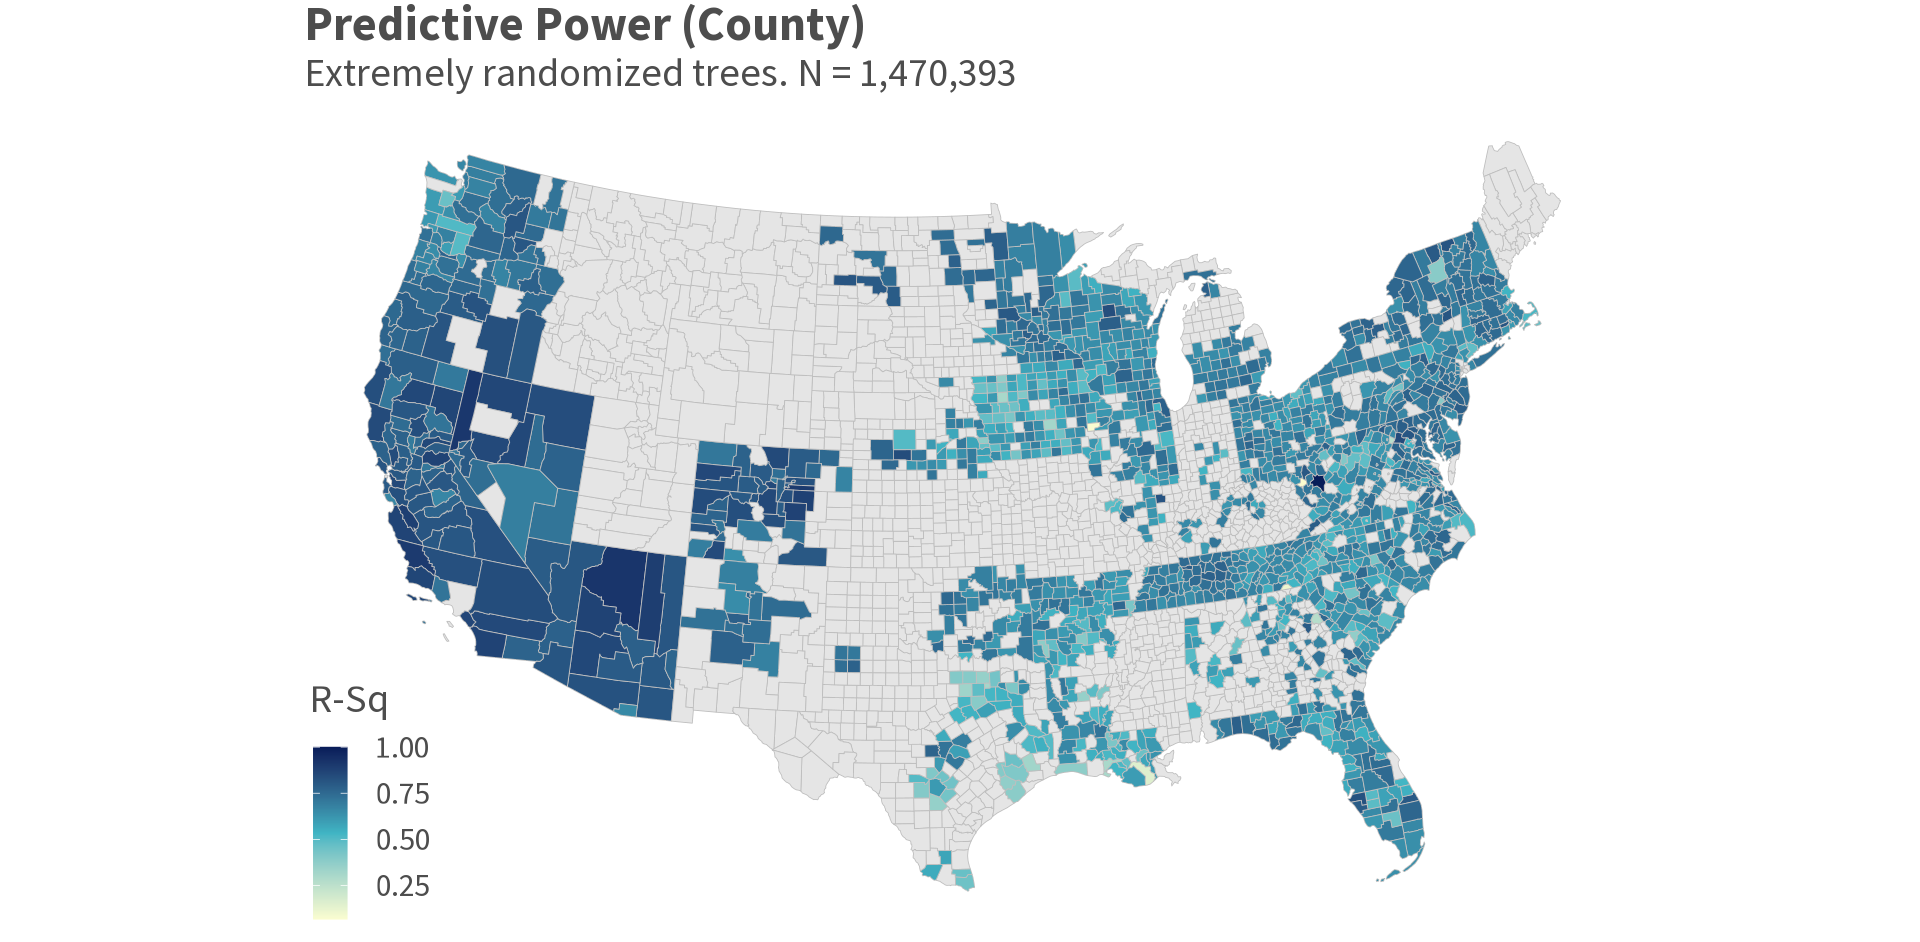
\includegraphics[width=6in]{figures/rf_rsq_map.png}
    \caption{Sales By County}
    \label{fig:rsq_county}
\end{figure}

\begin{figure}
    \centering
    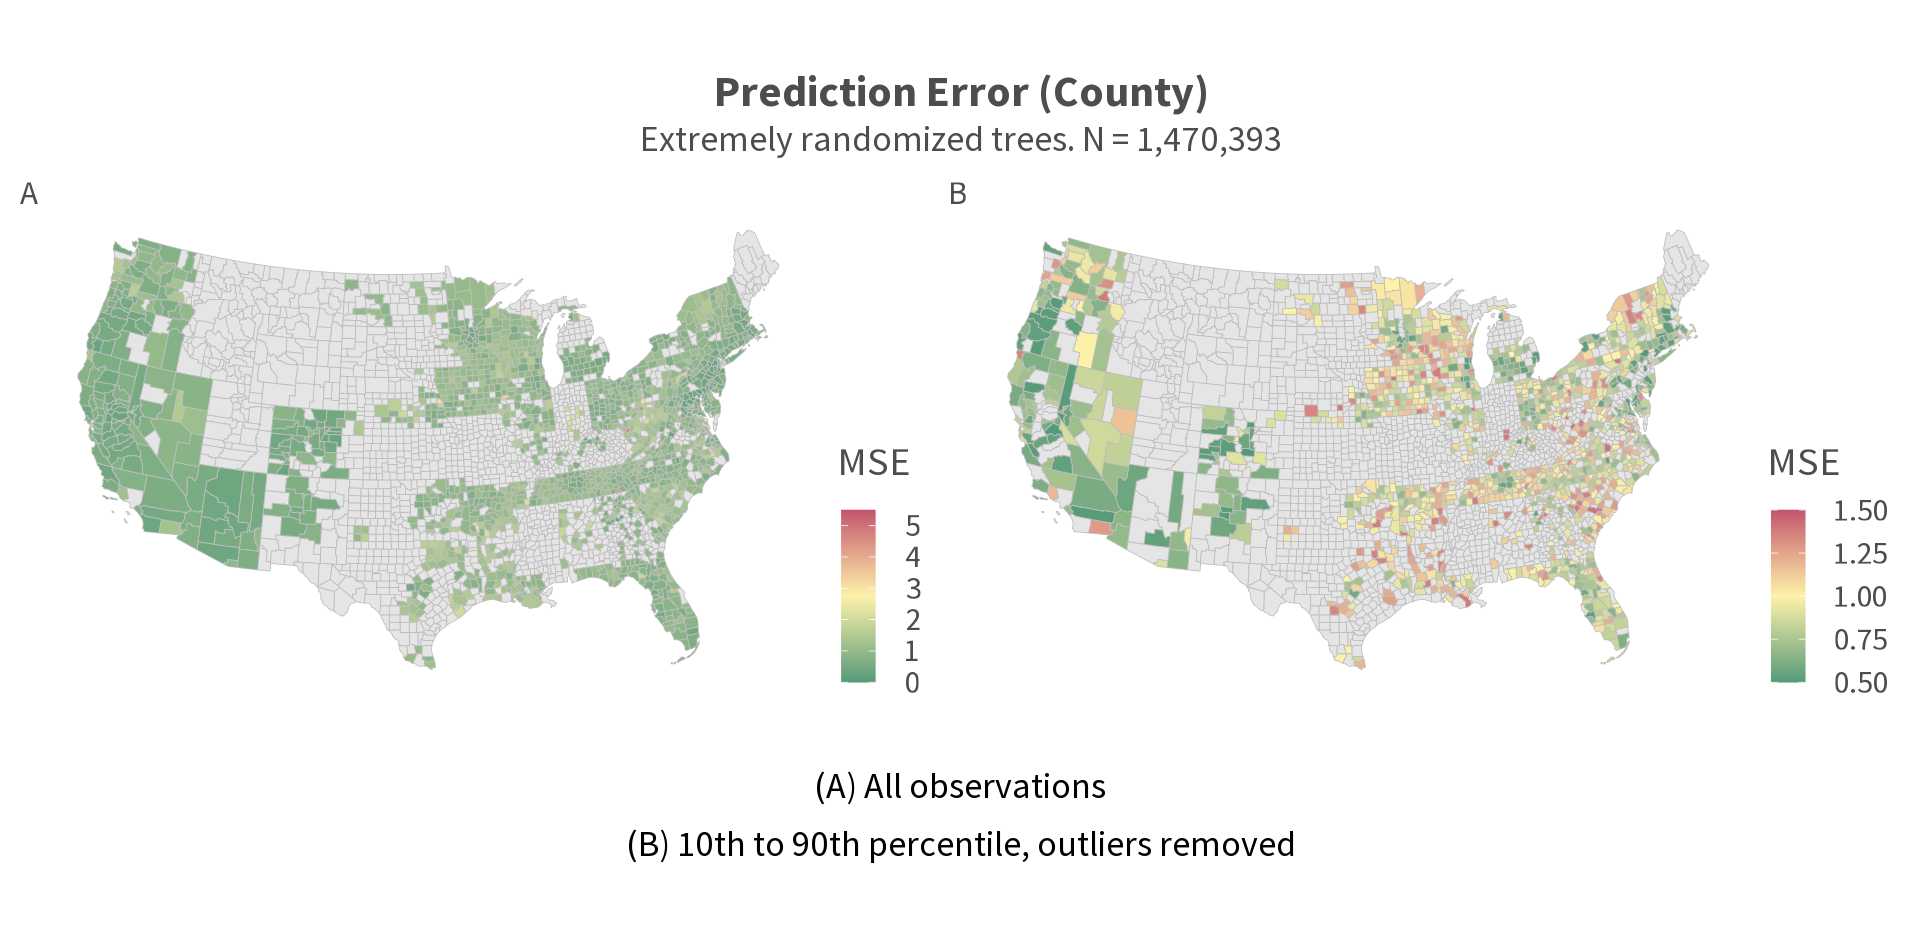
\includegraphics[width=6in]{figures/rf_mse_map.png}
    \caption{Model Performance: Prediction Error}
    \label{fig:mse_county}
\end{figure}

\newpage

\begin{figure}
    \centering
    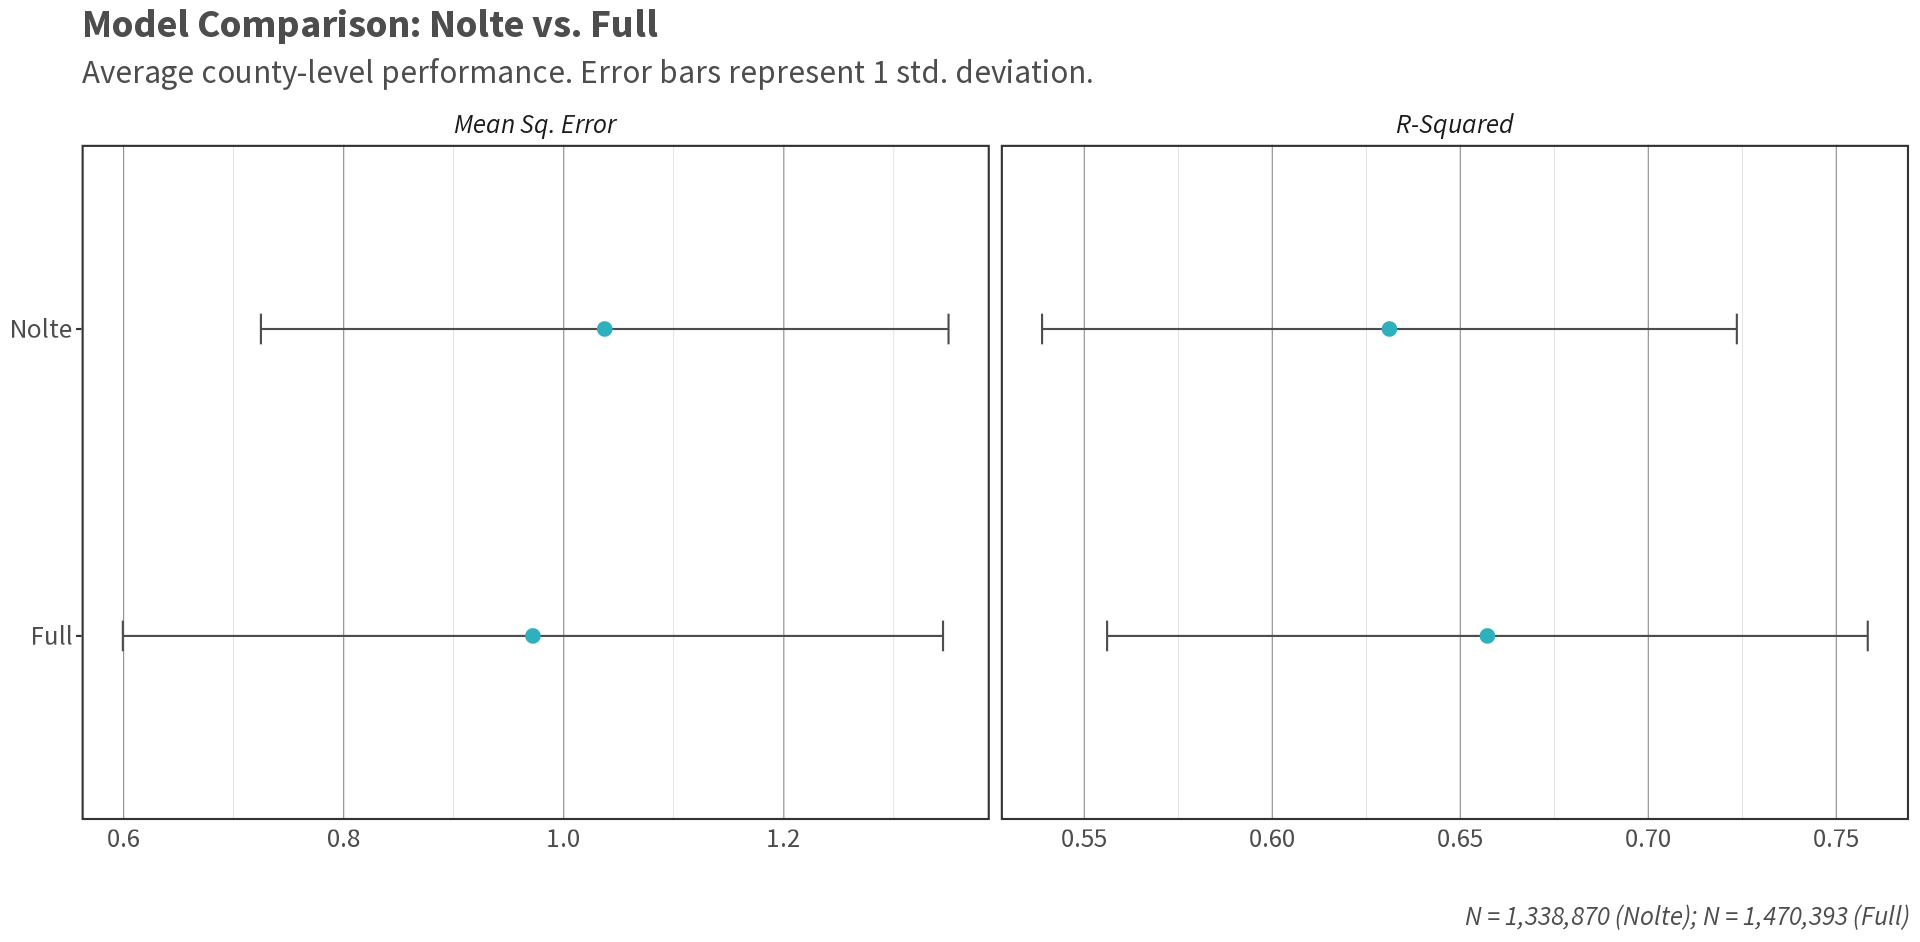
\includegraphics[width=6in]{figures/nolte_full_compare.png}
    \caption{Model performance: Only Nolte features vs. all features model}
    \label{fig:nolte_full_compare}
\end{figure}

\newpage

\section{Discussion}

DISCUSSION

\newpage

\section{Conclusion}

CONCLUSION

\newpage

\section{Appendix}


\subsection{Parcel filter}

\begin{enumerate}
    \item Meets ``undeveloped" criteria established by Nolte (2020), \textbf{or}
    \item Over half its area was classified as either grassland/herbaceous or planted/cultivated in the 2011 National Land Cover Database (NLCD), \textbf{or}
    \item Over half its area was classified as agricultural in the 2000 Land Change Monitoring, Assessment, and Projection (LCMAP), \textbf{or}
    \item Had any of the following ZTRAX land use codes:
    \begin{enumerate}
        \item Agricultural (``AG");
        \item Homestead (``MS113");
        \item Vacant open space/conservation/forest land (``VL104");
        \item Vacant agricultural/unimproved (``VL108")
    \end{enumerate}
\end{enumerate}

\subsection{Alternate Model Specifications}


\subsection{Multi-parcel Aggregation}



\newpage


\printbibliography

\end{document}